\documentclass[aps, pre, twocolumn, a4paper, floatfix]{revtex4}
%\documentclass[twocolumn]{revtex4}
\usepackage{graphicx}
\usepackage{amsmath}
\usepackage{placeins}
\usepackage{color}
\usepackage{hyperref}
%\usepackage{bug}
%\bibliographystyle{plain}
\newcommand{\er}{Erd\H{o}s-R\'{e}nyi}
\newcommand{\kk}{\langle k \rangle}
\newcommand{\red}{\color{red}}


\begin{document}

%\title{Avoidable colors percolation: Increasing security with heterogeneous paths}
\title{Secure message passing on networks with insecure nodes}

\author{Sebastian M. Krause}
\affiliation{Theoretical Physics Division, Rudjer Bo\v{s}kovi\'{c} Institute, Zagreb, Croatia}
\author{Michael M. Danziger}
\affiliation{Department of Physics, Bar Ilan University, Ramat Gan, Israel}
\author{Vinko Zlati\'{c}}
\affiliation{Theoretical Physics Division, Rudjer Bo\v{s}kovi\'{c} Institute, Zagreb, Croatia}
\begin{abstract}
It is often necessary to transmit a message across a network when parts of the network are not secure.
Here, we consider the case of a network partitioned into sets of nodes with the assumption that no single subset can be trusted.
As such, the message needs to be divided and transmitted on multiple paths so that no subset sees the entire message.
This problem arises, for instance, in a peer-to-peer (p2p) network running different unpatched software versions 
and when considering AS-level listeners in the entry and exit to the Tor network.

We present a general analysis of this problem on random graphs including analytic solutions for \er and scale-free networks and numerical simulations confirming our calculations and further numerical tests on real-world networks including the internet, partitioned by AS.

Surprisingly, we find that increased software heterogeneity may actually improve security.
\end{abstract}
%\pacs{89.65.-s, 05.50.+q, 05.65.+b, 64.60.De}
\maketitle


\section{Introduction}

Secure and anonymous communication over networks, in particular the internet, has become a central question facing the global community.
In light of widespread state-surveillance, large-scale cybercrime and superbugs like ``Heartbleed,'' one can no longer assume that an entire communications network is secure.

However, the network insecurity may be disjoint.  
For instance, on a p2p network, there may be different versions of the software running at the same time.  
In such a case, though there may be unpatched or even undiscovered bugs affecting a given version, it is unlikely that all of the versions will be compromised by the same group at the same time.
In such a case, a sensible strategy for secure communication may be to divide the message and transmit it along different paths so that \textit{no single version} receives the entire message.
With this heuristic, secure communication can be achieved even if large parts of the network are insecure.

This problem also arises when attempting to safeguard anonymity with the Tor network \cite{dingledine-proceedings2004}.  
Recent work has shown that if the same autonomous system (AS) controls a router on the path from the source to the entry node of the Tor network and also a router on the path from the exit node to the destination, the identity of source and destination can be deduced from a statistical analysis of the traffic pattern and the anonymity of the Tor network is broken \cite{murdoch-proceedings2007}.
Since a relatively small number of AS's control the entire internet, this scenario is a serious concern \cite{edman-proceedings2009}.
Indeed, we find that heterogeneity of management and versioning may provide higher levels of security.


\paragraph{Background}

{ \color{red} How exactly do Dolev and Pinto relate to our problem? }
In the 1990s, using sets of paths with disjunct servers \cite{dolev-acm1993}.
This early study, which gained broad attention in computer science [...],
abstracted from the network structure and assumed the existence of the paths a priori. 

The possibility of secure communication was studied as
well for wireless networks using percolation on spatially embedded
graphs \cite{pinto-ieee2012}. 


Here we examine this problem on general network topologies several partitioning rules.  
We do not consider here the implementation details of such a communication strategy but rather show under what circumstances it would be possible in principle.
We begin with a formal definition of the problem and its relationship to percolation theory and then proceed to demonstrate a number of key properties on random graphs and sample measurements on real-world networks, including the AS-level internet.

To analyze this problem, we consider a network for which each node is assigned exactly one color.
We assume that one of the colors is insecure but \textit{a priori} we do not know  which one.
Therefore, a pair of nodes is securely connectable iff there exist a set of paths connecting the nodes such that no color appears on all of the paths.  
This property suggests an analytic approach similar to percolation theory on networks.
If node or link failures occur with a given probability, 
percolation theory on complex networks can be used to determine overall connectivity \cite{cohen-book2010,newman-book2010}. 
{\color{red} Do we use $k$-core percolation? If not, why do we need to discuss it?}
In particular, $k$-core percolation \cite{dorogovtsev-prl2006} has interesting implications due to the special k-core structure of the AS server network of the
Internet \cite{tauro-ieee2001,carmi-pnas2007}. 


%However, recent security problems where often due to gaps in
%the software, and therefore whole sets of servers will likely fault at
%the same time, if they use the same software version of the OS, transmission
%software etc.

To calculate the probability of secure communication, we develop a new kind of percolation theory in which topological connectivity alone is not a sufficient condition.
Rathar, a pair of nodes is connectable if there exists a set of paths between them, each of which avoids one of the colors in the system.
There may be a smaller set of paths which securely connects the pair of nodes but such a case is trivially included in the condition of connectability via a maximal number of paths.

%
%this property we begin by examining color-avoiding connected components.
%For every color $c$, the color avoiding component is defined as all nodes which can be reached when the $c$-colored nodes are removed.
%
%
%
%Here we analyze how the secret sharing method can be used to send
%messages in a secret way, even if one software version is faulty and it is
%not known which one. 



\section{Avoidable colors percolation}

\begin{figure}[htb]
\begin{center}
    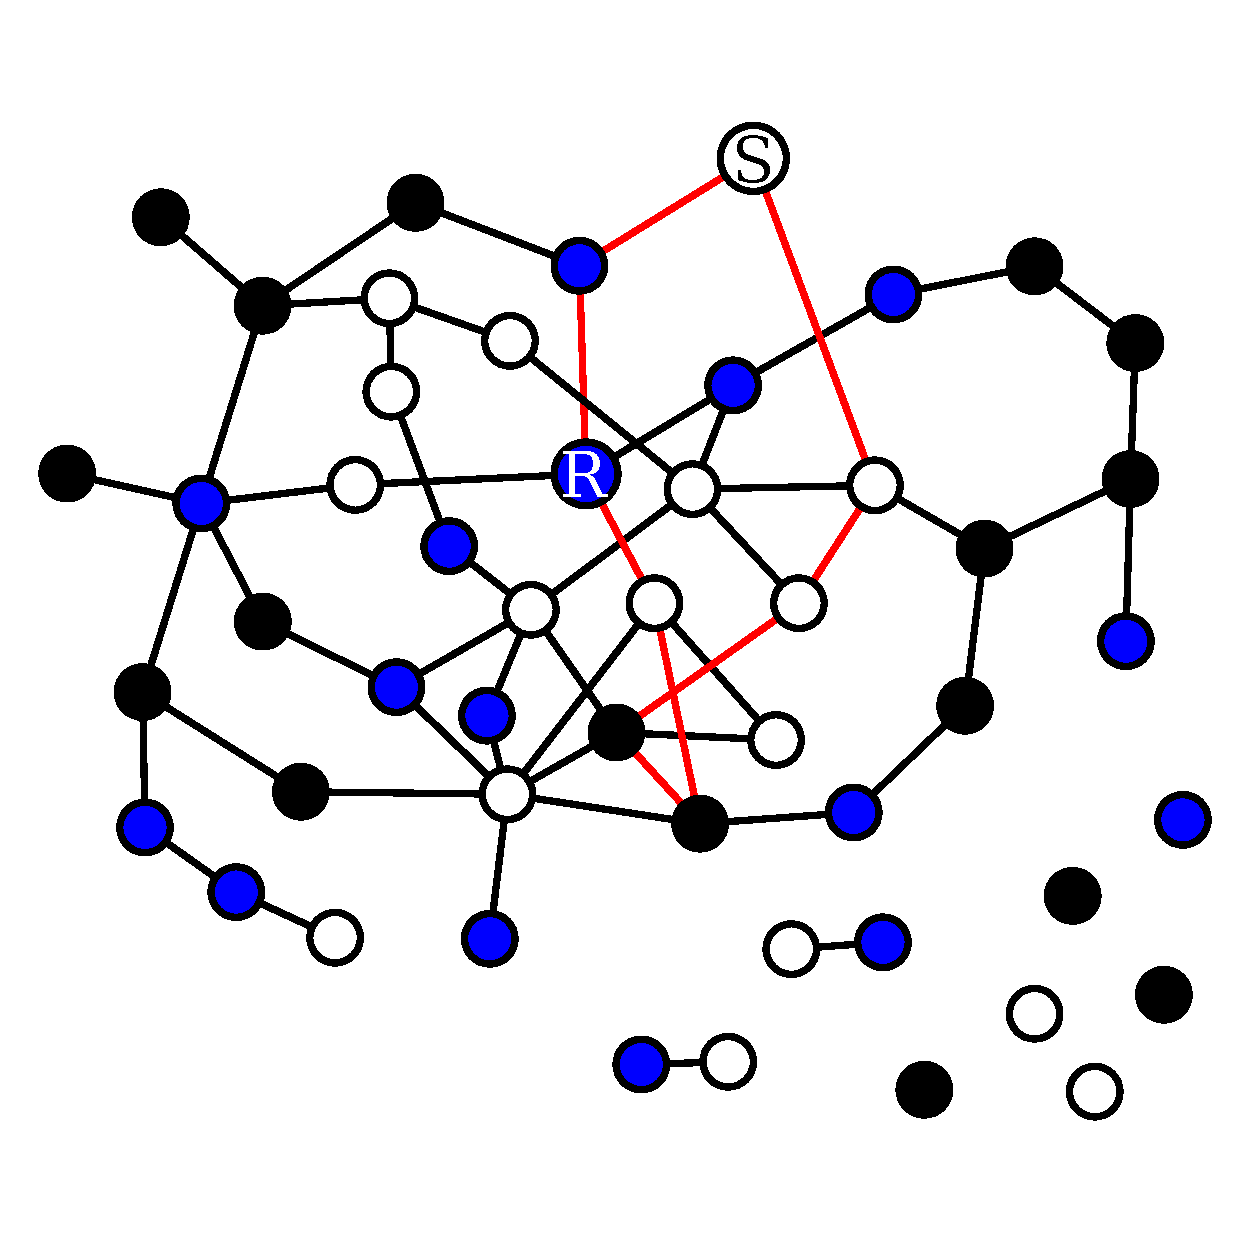
\includegraphics[width=0.49\columnwidth]{graph_sr.pdf}
    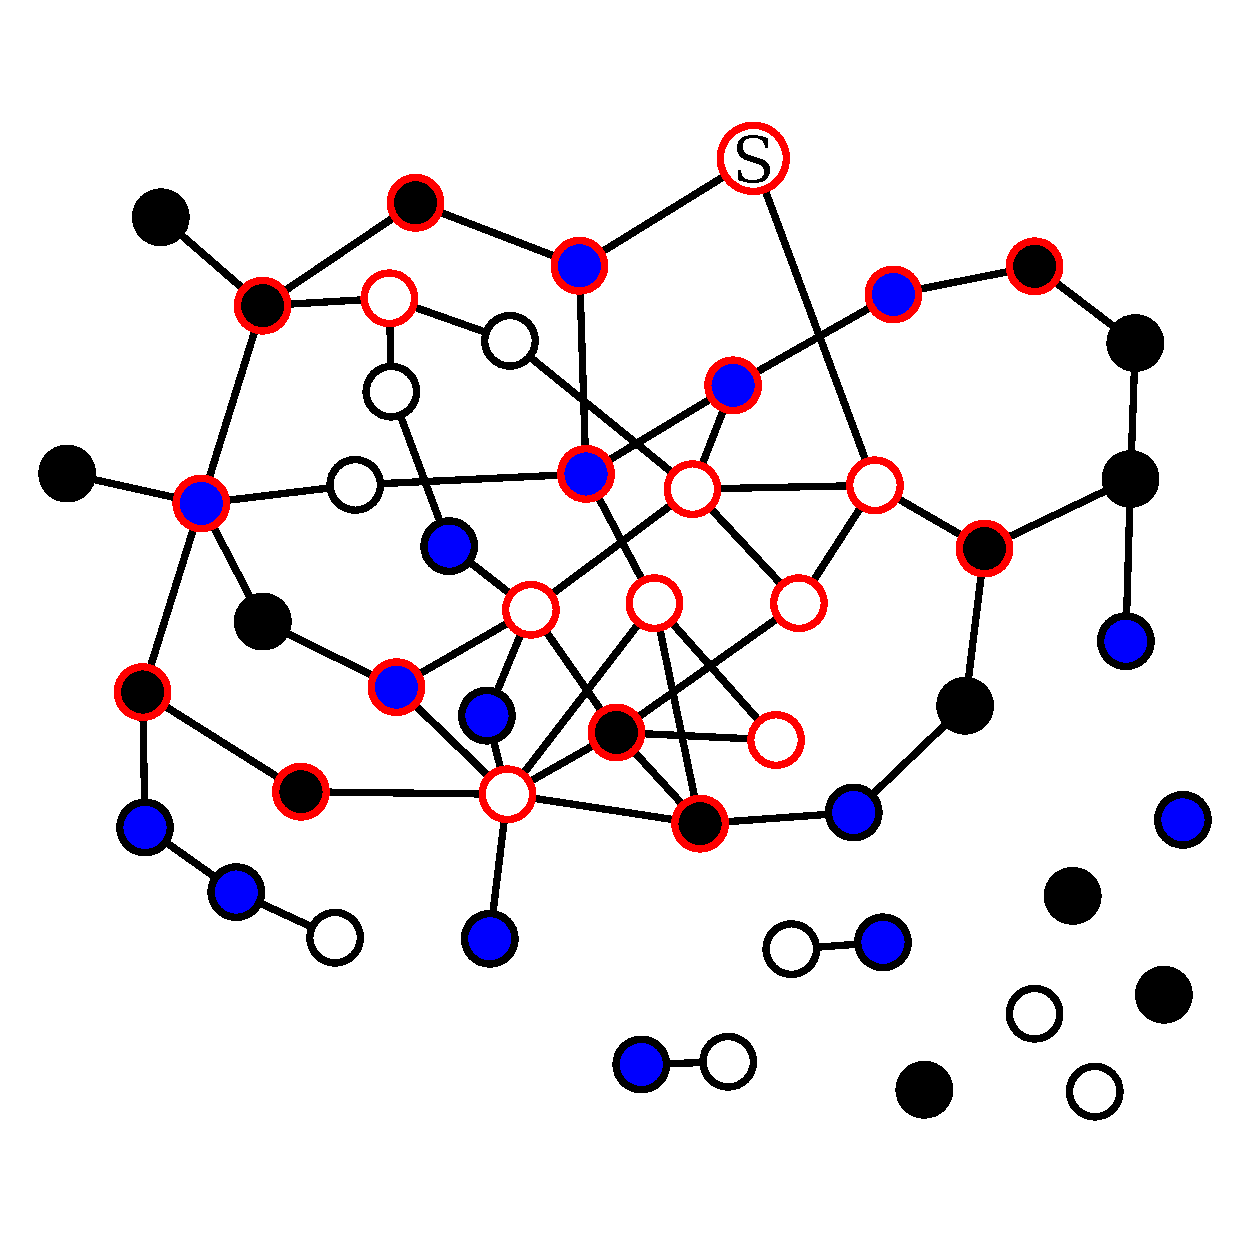
\includegraphics[width=0.49\columnwidth]{graph_Gcolor.pdf}
    \caption{Left: In this network the sender S and the receiver R can communicate 
    with avoidable colors, as the short path highlighted with red avoids black and 
    white nodes, and the long path avoids blue nodes. Right: All nodes highlighted 
    with red belong to an avoidable colors component, as each pair out of this set 
    is connected with avoidable colors. Notice that some nodes which are needed 
    for connection of other nodes are not included in the component.}
    \label{fig:avoidable_colors}
\end{center}
\end{figure}
%
Assume a graph $G$ with $N$ vertices and adjacency matrix $A_{ij}$. Every vertex 
$i$ has a color $c_i\in\{1,2,\dots,C\}$, where $C$ denotes the total number of colors. 
The colors may stand for software versions on servers, where all servers of the 
same version are likely to fail at the same time; 
they may stand for ownership/control, where the controlling body (company, government etc.) may be assumed to eavesdrop on their nodes;
they may stand for economic entities with correlated failure probability (due to financial dependence, reliance on the same resource); 
or they may stand for reloading points of transportation (e.g. ports with transferring goods from ship to train, where strikes could hit many ports at the same time). 
Faced with the possible collective failure or insecurity of all nodes of a single color, 
``connectivity'' means that two nodes are required to be ``connected with avoidable colors'': 
For every color $c$, a connecting path must exist, such that \textit{all} nodes 
on the path are \textit{not} of color $c$. This is illustrated on the left of 
figure~\ref{fig:avoidable_colors}. 
In the following, we refer to this property as ``color-connected.''

In order to discuss the connectivity of the network in general, 
we define an ``avoidable colors component'' as a maximal set of nodes, 
where every node pair is connected with avoidable colors. 
Such a component is highlighted with red in Fig. \ref{fig:avoidable_colors}. 

{\red 
Note that there are nodes needed for providing 
connections which themselves do not belong to the avoidable colors component. 
\textit{This is a very interesting property. We should discuss it more thoroughly.}}

By studying the avoidable colors component, we obtain a clear quantitative measure of the feasibility of security through multiple-path routing and information on where those paths should be routed.
Furthermore, this gives us a way to measure the effect of changes in network topology, link density, number of colors and the color distribution.

%Labeling avoidable colors components can be useful for different tasks: 1) The 
%fraction of nodes being in the largest avoidable colors component tells us whether 
%it would be useful to implement real world routing algorithms (if only a tiny fraction of 
%servers in the Internet is able for avoiding colors, it is not worth of thinking about 
%new protocols). 2) By highlighting the nodes which are connected with many others with 
%avoidable colors, routing algorithms can save time by not searching for impossible 
%connections. 3) The positive effect of adding links, moving colors or increasing color 
%heterogeneity can be quantified and balanced with possible costs or regulation issues. 

\begin{figure}[htb]
\begin{center}
    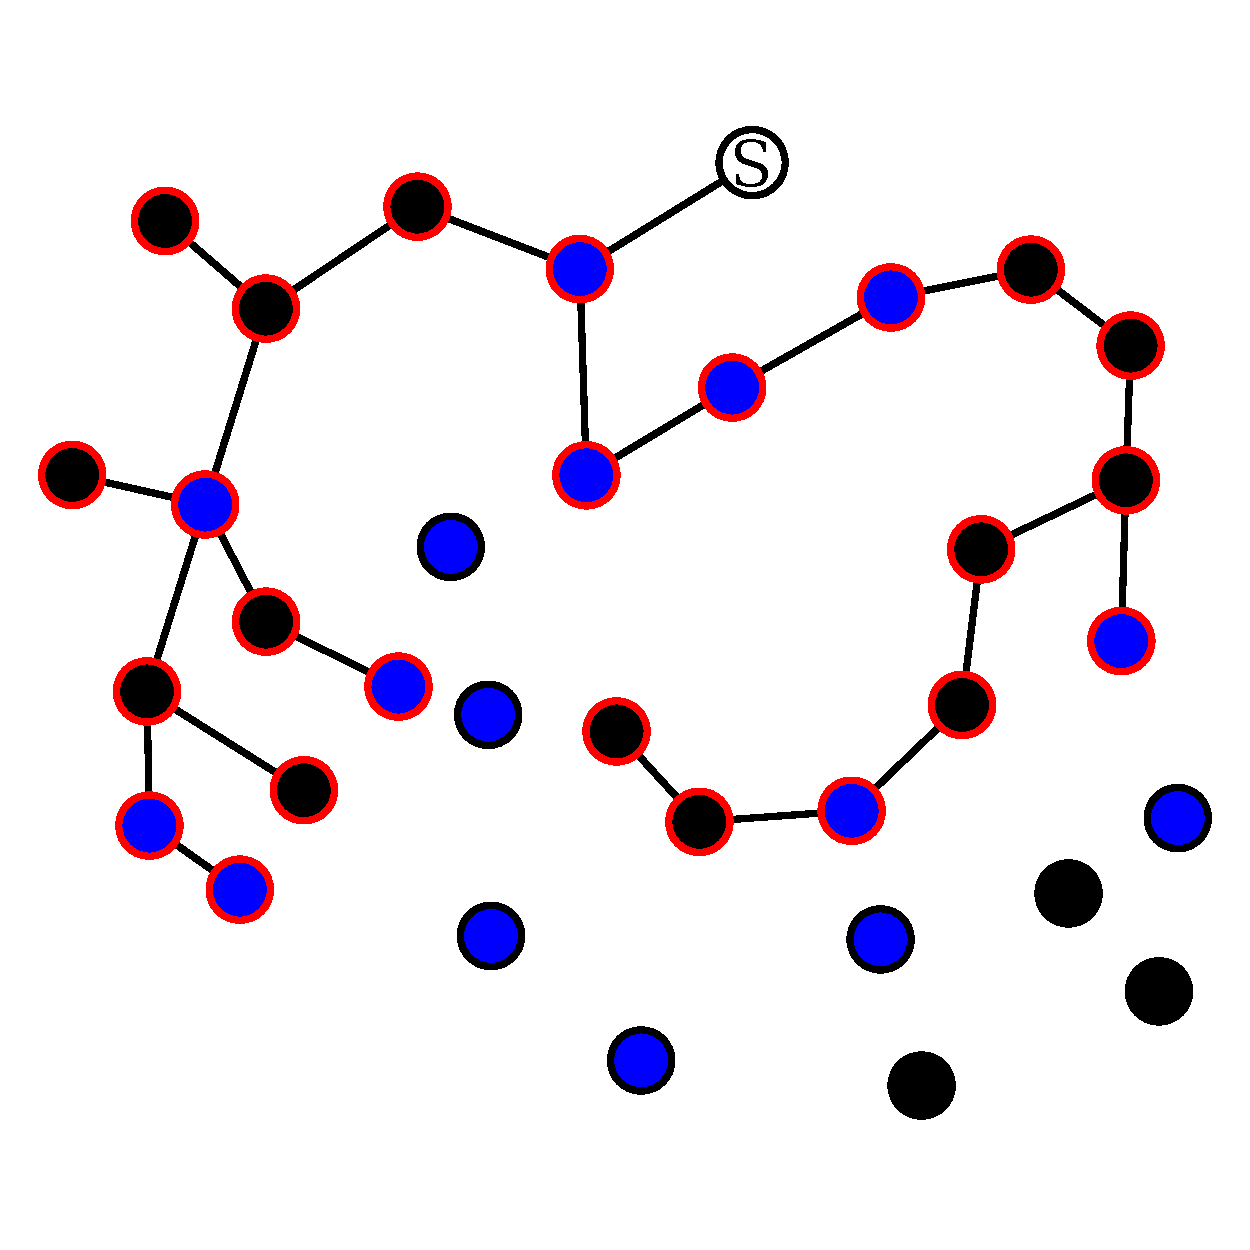
\includegraphics[width=0.45\columnwidth]{graph_avoid0.pdf}
    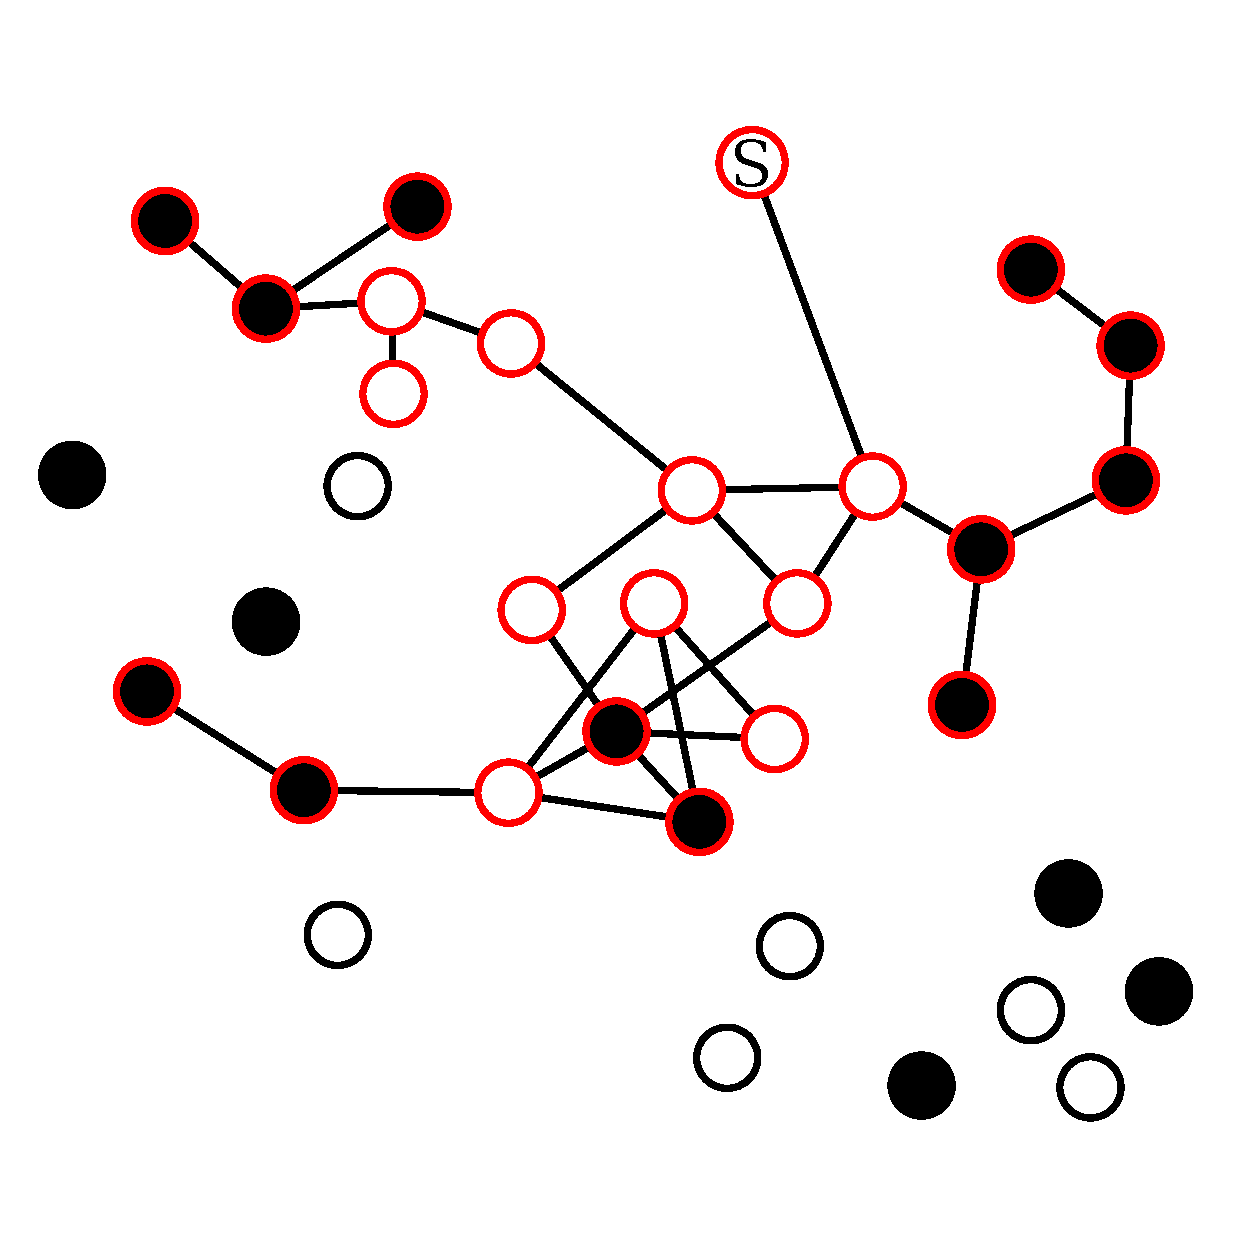
\includegraphics[width=0.45\columnwidth]{graph_avoid1.pdf}
    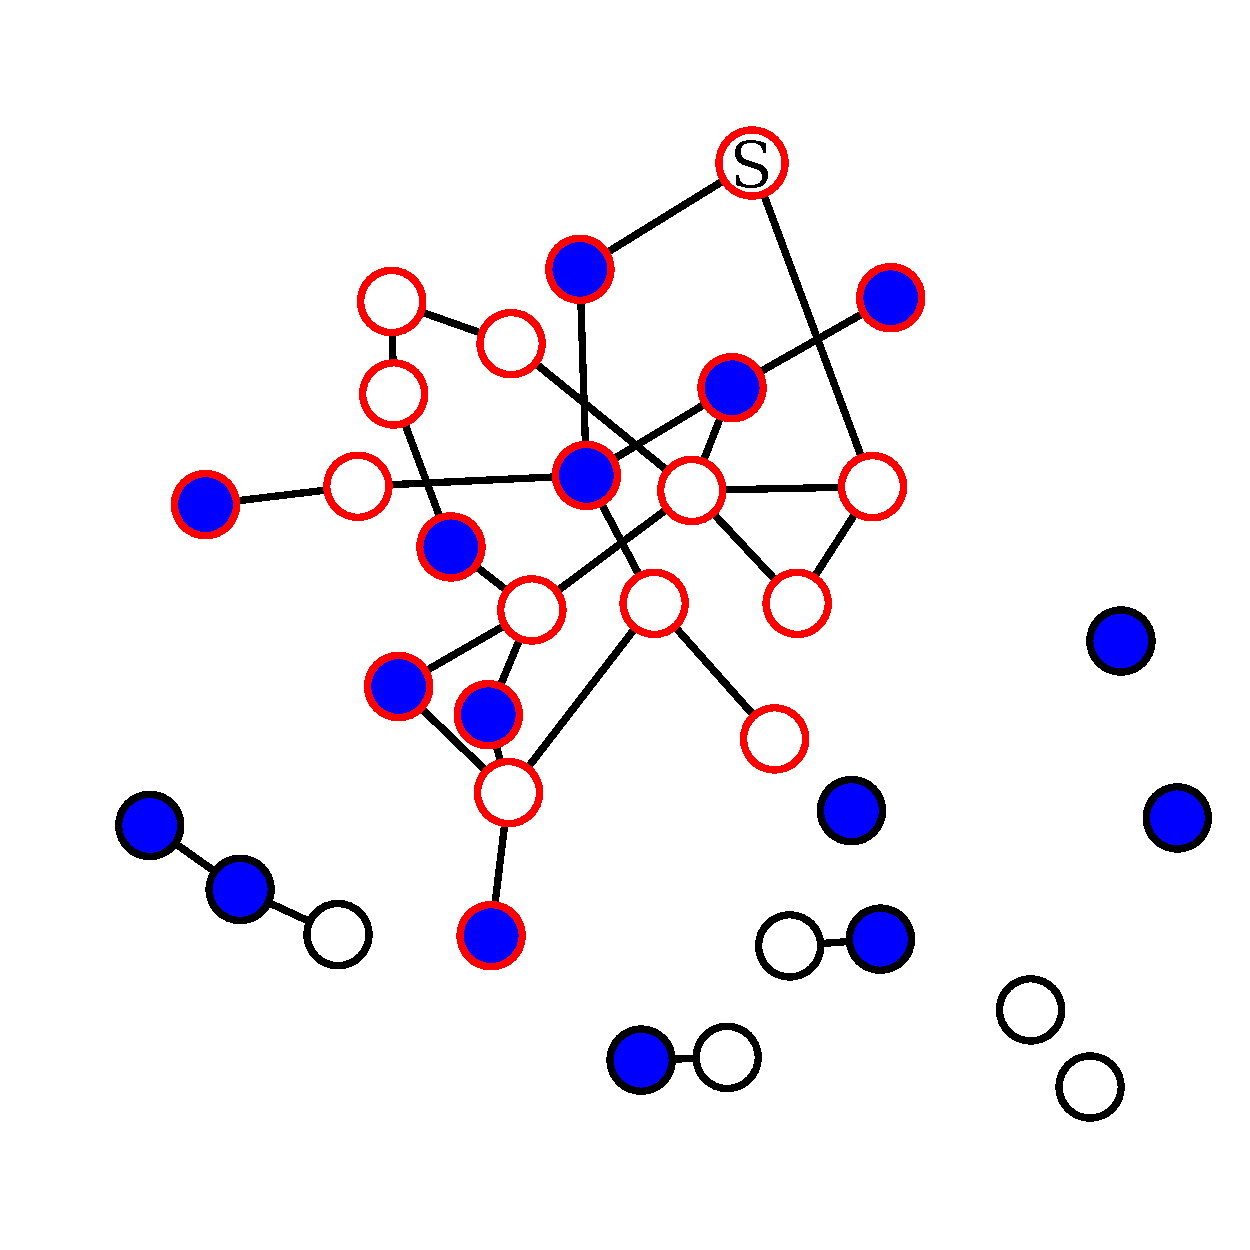
\includegraphics[width=0.45\columnwidth]{graph_avoid2.pdf}
    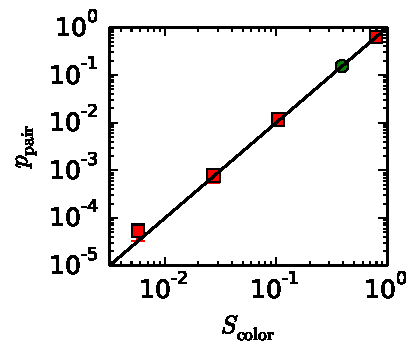
\includegraphics[width=0.53\columnwidth]{pairs_S_color.pdf}
    \caption{Illustration of the construction of the  set of nodes $L_{\rm color}$ which is the largest avoidable colors component {\red \textit{I don't understand.  Why many?} in many large networks. }
    The largest components without white ($L_{\bar 1}$), without blue ($L_{\bar 2}$) and without 
    black nodes ($L_{\bar 3}$) are highlighted in red, and the test node S is connected to 
    all of them and therefore belongs to $L_{\rm color}$. Lower right: Estimation of the fraction 
    of successful pairs for quenched graphs with different values $S_{\rm color}=N_{\rm color}/N$. 
    Red squares show Poisson graphs with increasing degree and $C=3$ colors, the green circle 
    shows the autonomous systems network with $C=2$ colors. The black line indicates the case 
    where only node pairs in $L_{\rm color}$ are connected with avoidable colors. As numerical 
    results are close, $L_{\rm color}$ indeed dominates the secure communication abilities of many
    graphs.
    Notice that even for the smallest value shown, $N_{\rm color}=570$ has reasonable size. The blue circle shows the network of autonomous systems with two colors distributed over the nodes. Our network 
snapshot of the year 2006 contains $N=22963$ nodes. $p_{\rm pair}$ was approximated with 
samples of up to $5\times 10^5$ pairs, error-bars are smaller than the symbols in most 
of the cases. 
    }
    \label{fig:avoidable_colors_candidate}
\end{center}
\end{figure}
%
As illustrated in figure~\ref{fig:avoidable_colors_candidate}, 
there is a way to find a candidate set of nodes $L_{\rm color}$ 
for the largest avoidable colors component.
First, for every color $c$, we delete all nodes with color $c$ 
and find the largest component in the remaining graph, $L_{\bar c}$. 
Next, we define $L_{\rm color}$ as the set of nodes such which are in $L_{\bar c}$ or have at least one link to it; for every color $c$. 
Now every node pair in $L_{\rm color}$ are color-connected. 
{\red \textit{I don't understand why this makes it maximal...}
If for every color $c$, $L_{\rm color}$ includes at least one node out of $L_{\bar c}$, 
it is maximal and therefore it is an avoidable colors component. }
There is no easy way to test whether $L_{\rm color}$ is the largest avoidable colors component 
(as shown in figure~\ref{fig:avoidable_colors_cases}, avoidable colors components can exist due to 
different mechanisms and they can largely overlap). 
However, we will see that $L_{\rm color}$ {\red \textit{This needs to be explained.} might} scale with system size 
and in this case it can be considered as a giant avoidable colors component. 
Letting $N_{\rm color}$ equal the number of nodes in $L_{\rm color}$,
we find that at least $N_{\rm color}(N_{\rm color}-1)/2$ out of all $N(N-1)/2$ 
possible node pairs in the network are connected with avoidable colors. 
This is a macroscopic fraction if $L_{\rm color}$ scales linearly with system size. 
{\red We can use this fact to test whether $L_{\rm color}$ dominates the secure communication abilities 
of a network by plotting the fraction of pairs connected with avoidable colors in the 
whole network $p_{\rm pair}$ against $S_{\rm color}=N_{\rm color}/N$. 
In figure~\ref{fig:avoidable_colors_candidate} on the lower right we see that secure 
connectivity is indeed dominated by $L_{\rm color}$. 
With red squares, results for Poisson graphs with $N=10^5$ nodes and average degrees 
${\bar k}=1.6;\,1.7;1.9;4.0$ are shown, where $C=3$ colors were distributed over the nodes 
uniformly at random. 
\textit{What are the other ways that color-secure communication can take place? Why does the deviation remain small? There's a piece missing here.}}
Results fit well even for small $S_{\rm color}$. 
This validates the treatment of $L_{\rm color}$ as a proxy for color-connectivity and allows us to develop analytical results and understand the system's critical behavior, as discussed below. 
%As we have seen that $L_{\rm color}$ may describe random networks and the real world 
%example of autonomous systems, we will base a theory for calculating the size of 
%the giant avoidable colors component on that idea. 



\begin{figure}[htb]
\begin{center}
    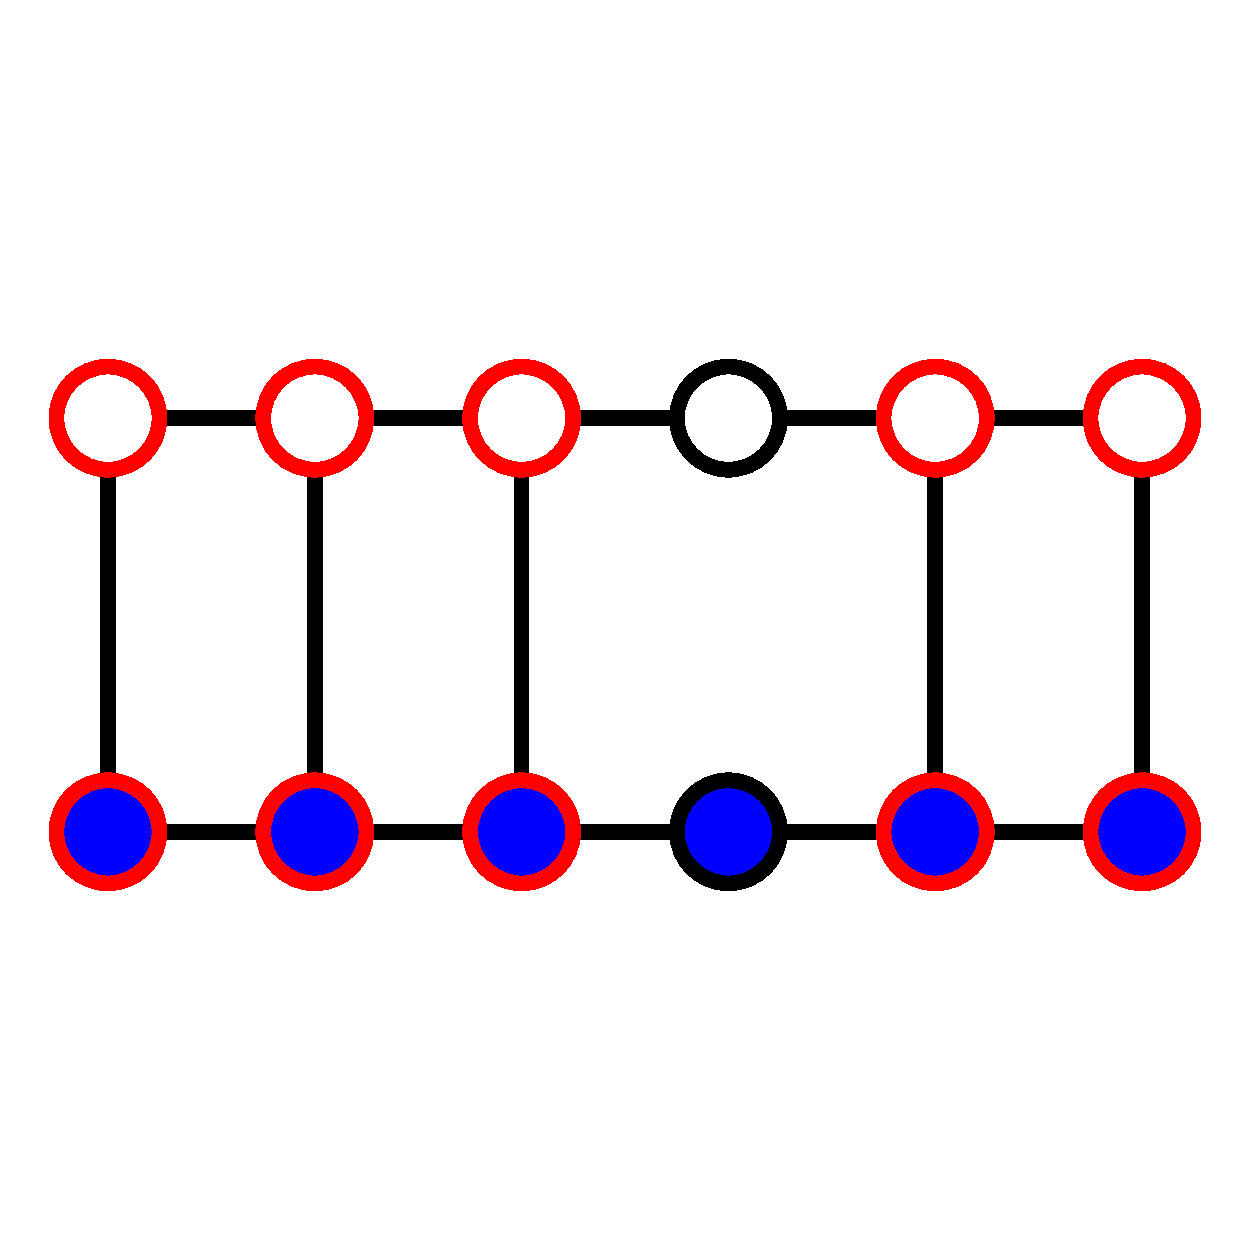
\includegraphics[width=0.18\columnwidth]{graph_1.pdf}
    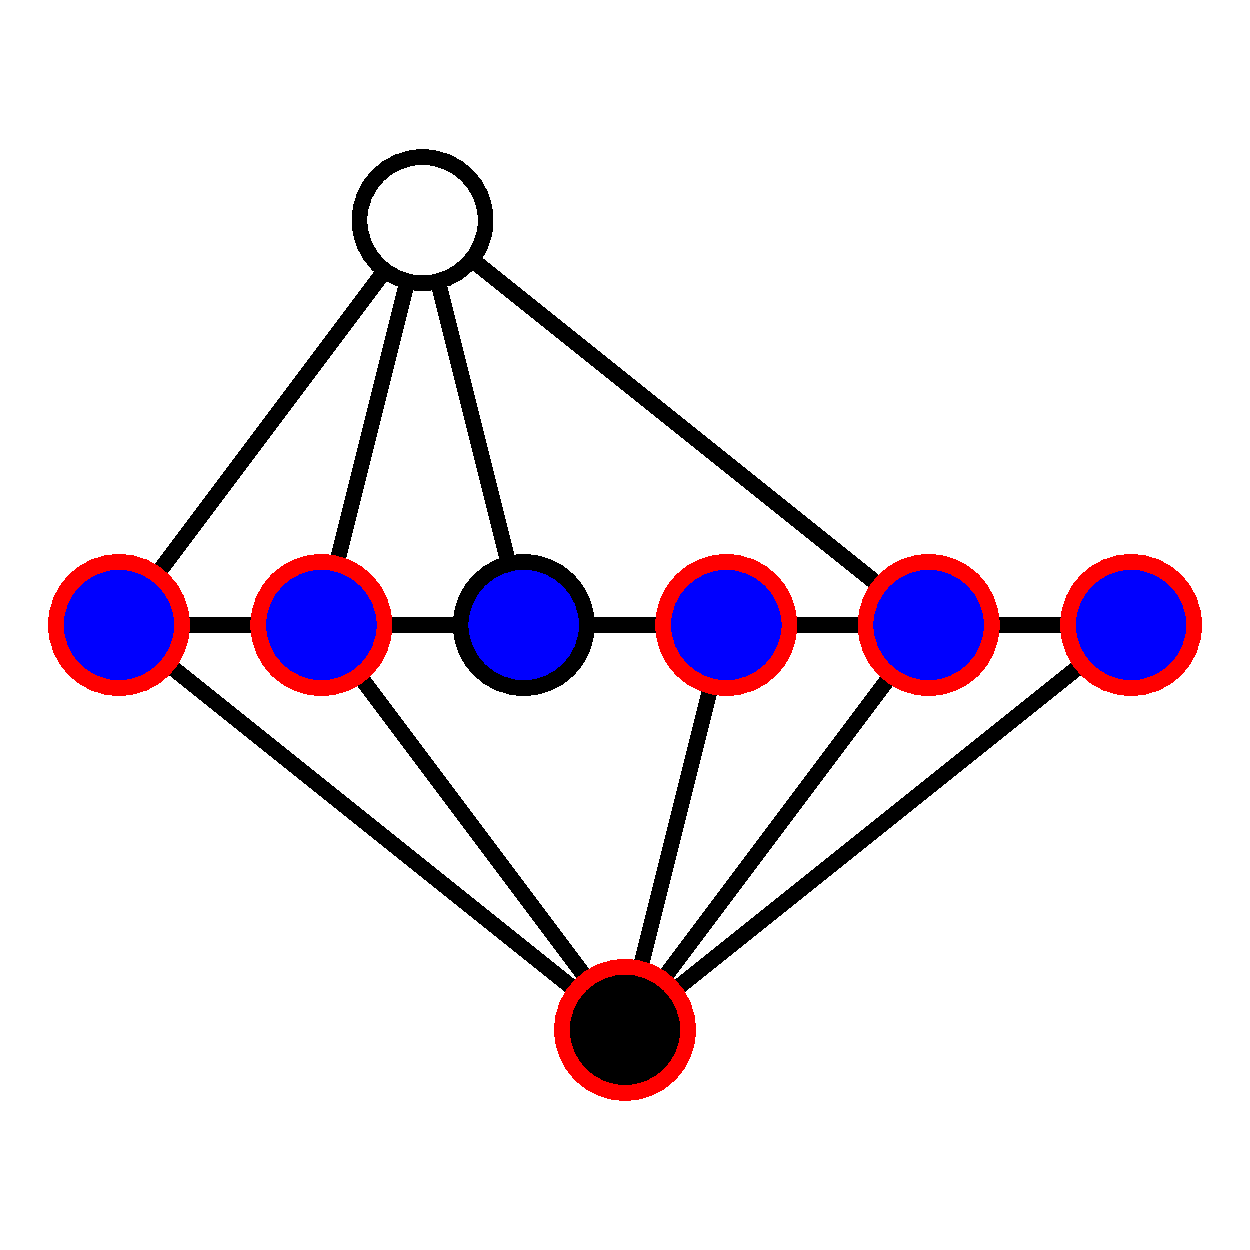
\includegraphics[width=0.18\columnwidth]{graph_3.pdf}
    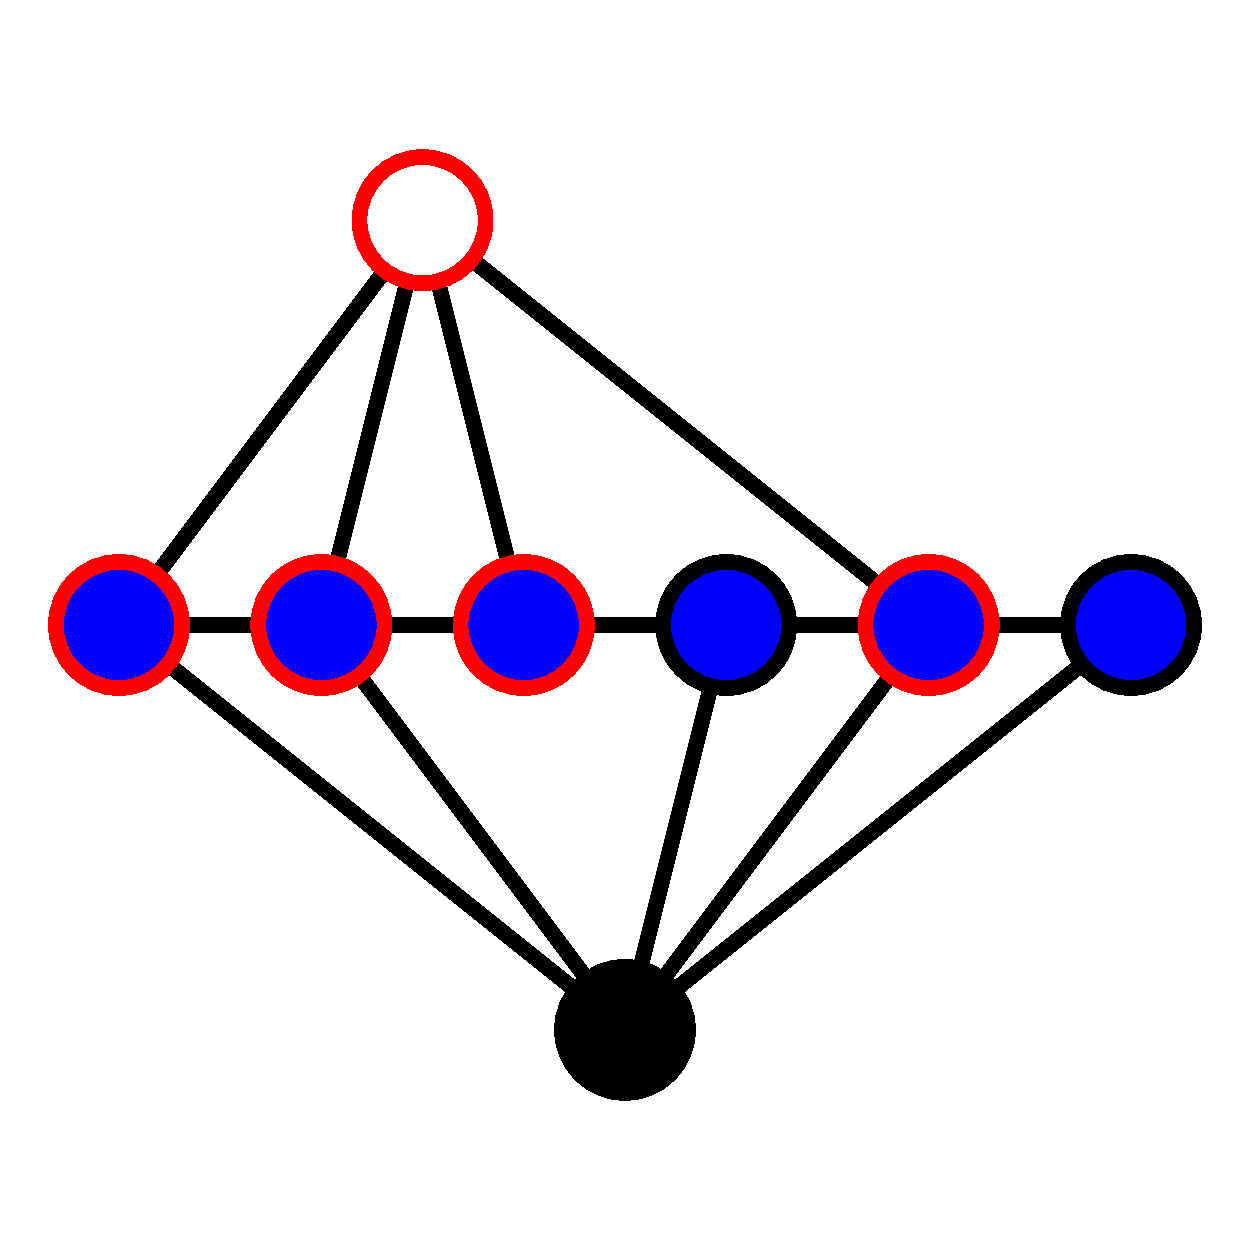
\includegraphics[width=0.18\columnwidth]{graph_2.pdf}
    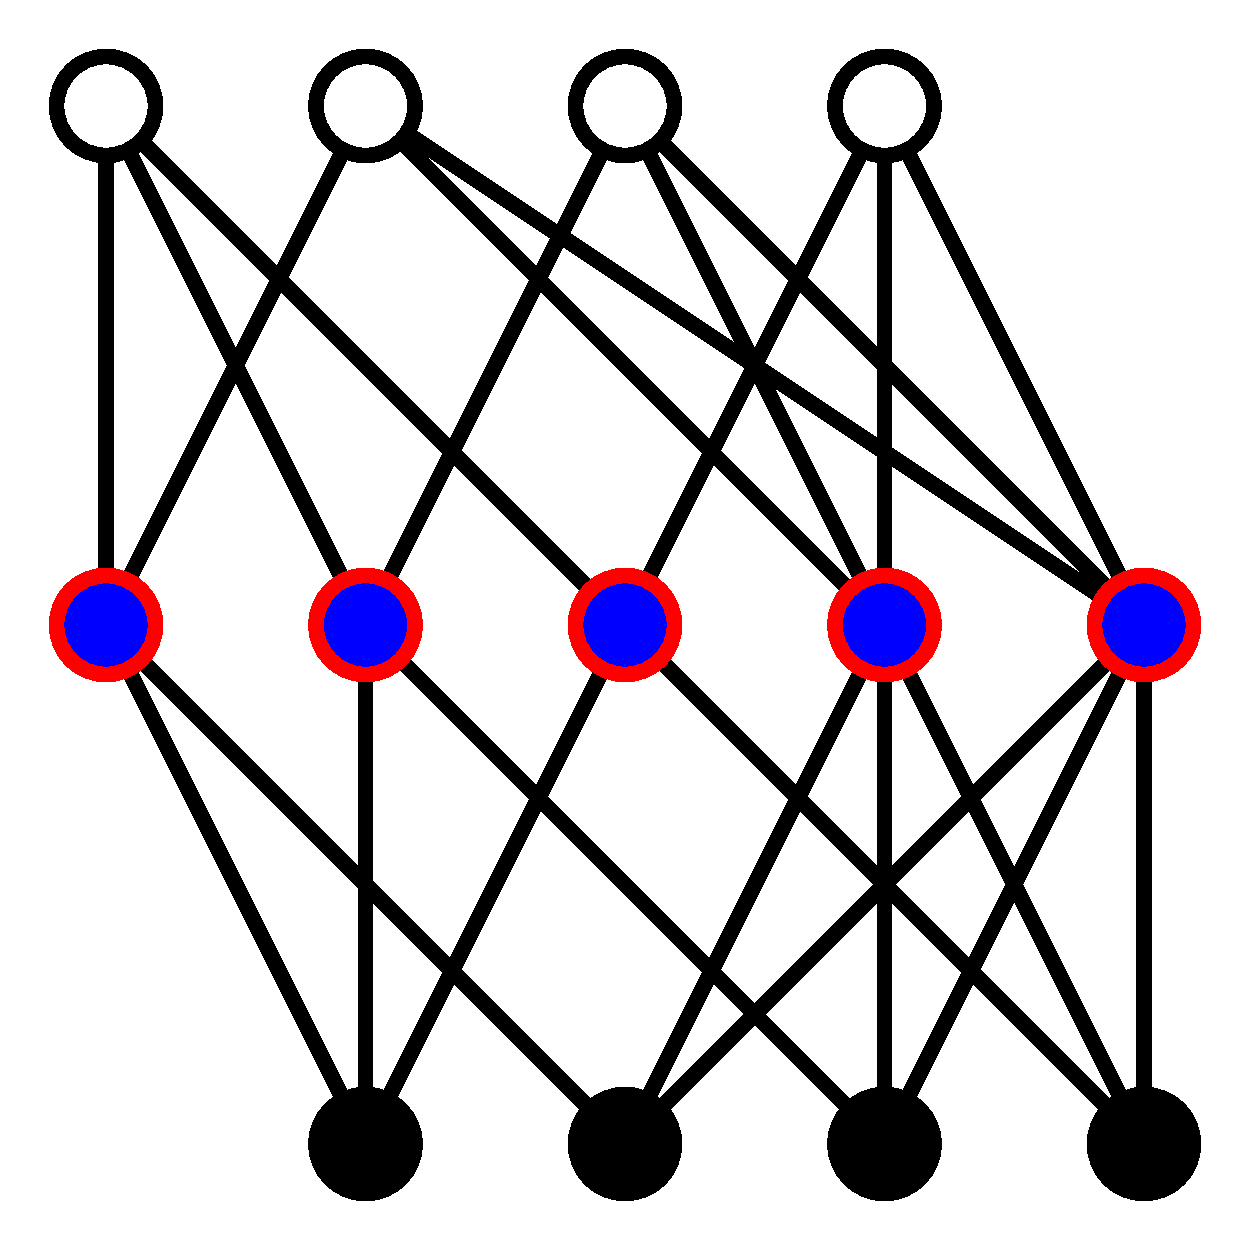
\includegraphics[width=0.18\columnwidth]{graph_4.pdf}
    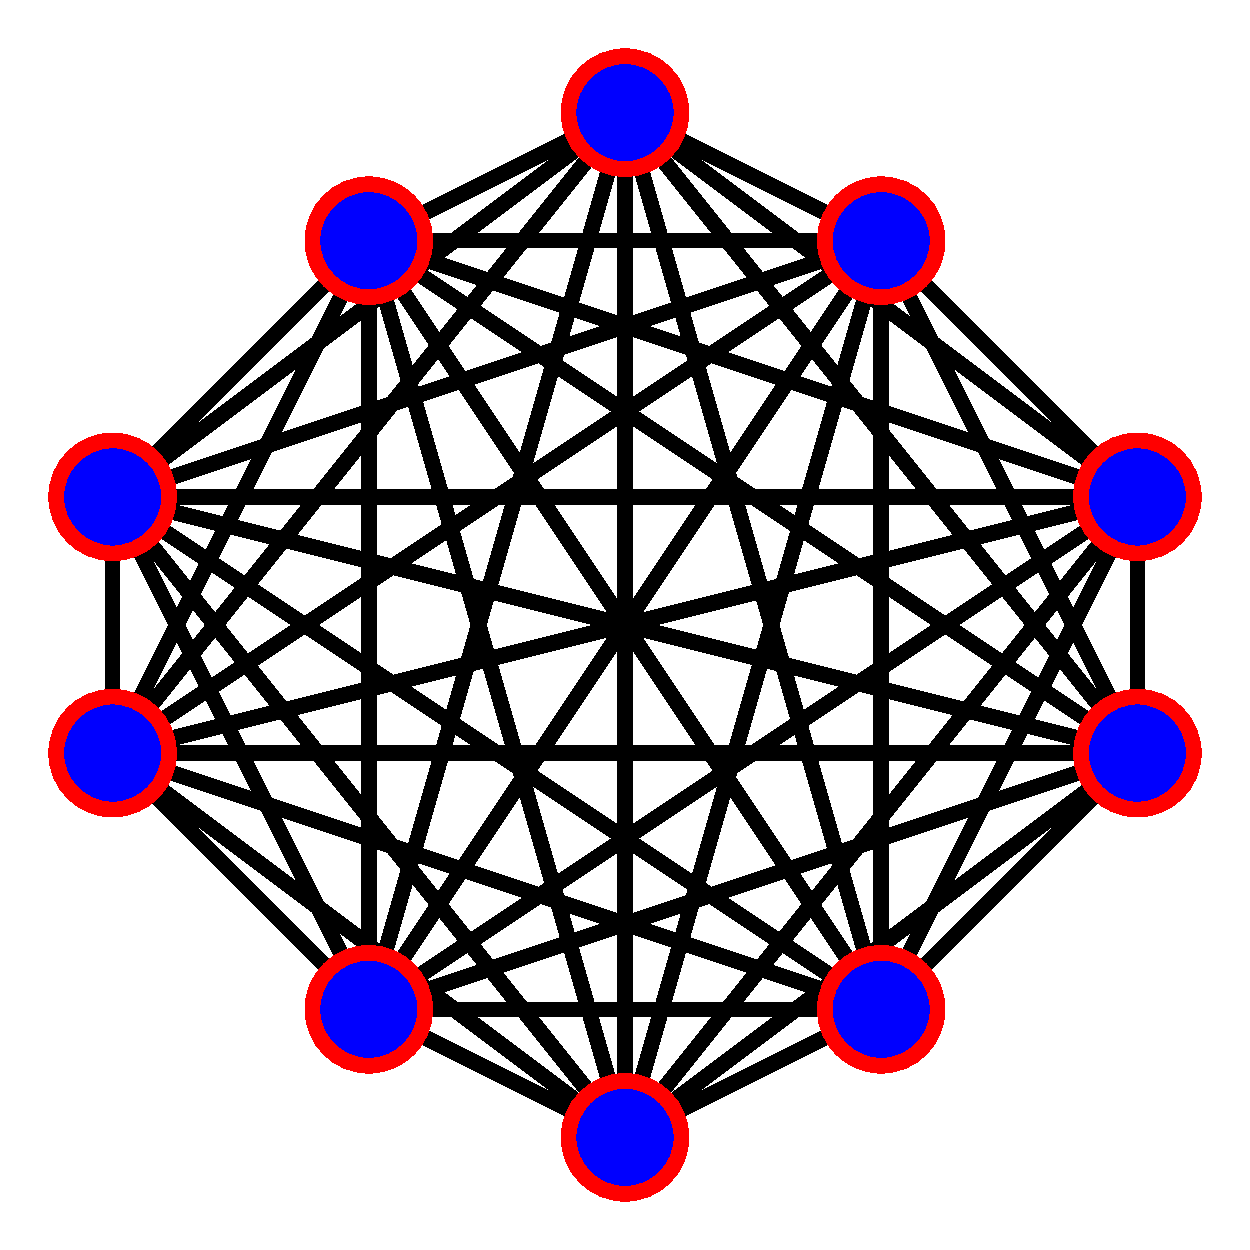
\includegraphics[width=0.18\columnwidth]{graph_5.pdf}
    \caption{{\red These should probably be subfig-ed and labeled.}
    Avoidable colors components, as highlighted with red, can be due to different 
    scenarios. 
    On the left, we see a {\red \textit{What makes this case scalable?} scalable} case similar to random graphs. 
    In the second graph, the high degree black node serves as an alternative paths provider for the blue nodes. 
    In the third graph an alternative avoidable colors component is highlighted for that 
    graph, showing that components might overlap. 
    The second graph from the right does not need any connection among the blue nodes 
    but there is a massive overhead of nodes and connections. 
    On the right, we see that a clique is an avoidable colors component by definition.}
    \label{fig:avoidable_colors_cases}
\end{center}
\end{figure}
%
To illustrate the rich phenomenology of avoidable colors components,  
some different mechanisms are shown in figure~\ref{fig:avoidable_colors_cases} 
which establish such components.
On the left, we see a case which is similar to  random graphs: 
all nodes which are neighbors to largest components without 
the color white and without the color blue can connect securely. 
{\red
In the second graph, the black node serves as an alternative paths provider for the blue nodes. 
It needs to have high degree for that. 
In the third graph an alternative avoidable colors component is highlighted. 
This shows that they might overlap and it is not straight forward to find the largest 
one. \textit{Evidently, color-communication does not work with such components.  How is this consistent with our understanding of the role of $L_{\rm color}$?}
The second graph from the right does not need any connection among the blue nodes 
and the connecting white and black nodes have lower degree, 
however, there is a massive overhead of nodes and connections. 
On the right, we see a clique. In this case, no node 
of a different color is needed for all nodes to be color-connected, but the number of links needs to be maxmial.




\section{Results}

We can find analytical results for random graph ensembles with randomly distributed 
colors in the limit of infinite graphs. The detailed derivation and explanation 
can be found in the supplements. We use the generalized configuration model graph 
ensemble with $N$ nodes, where each degree sequences $\{k_i\}$ occurs with probability 
$\prod_i p_{k_i}$ with the degree distribution $p_{k}$. Additionally we want to assign to 
every node $i$ a color $c_i\in 1,2,\dots,C$. For given degree sequence $k_i$, the color 
sequence $\{c_i\}$ has probability $\prod_i {\tilde r}_{c_i,k_i}$ with the degree-dependent 
color distribution ${\tilde r}_{c,k}$ ($\sum_c {\tilde r}_{c,k}=1$ for every degree $k$ 
separately). 

We calculate $S_{\rm color}$ in the limit of $N\to \infty$ as the probability of a 
single node to belong to $L_{\rm color}$. This problem can be decomposed into two parts. 
First, all possible cases of neighborhoods are summed over with the according 
probabilities. We need to specify the numbers $\kappa_c$ for all colors $c$. $\kappa_c$ 
counts the number of neighbors having color $c$ and at the same time being in the normal
giant component. Second, with the vector ${\vec \kappa}=(\kappa_1,\dots,\kappa_C)$, the conditional 
probability $P_{\vec \kappa}$ that these links suffice to connect to $L_{\rm color}$ can 
be calculated. This can be realized as follows:
%%%
\begin{align}
S_{\rm color} &= \sum_{k=0}^{\infty}p_k \sum_{k'=0}^{k} B_{k,k'} 
\sum_{\kappa_1,\dots, \kappa_C=0}^{k'} M_{k',\vec \kappa} 
P_{\vec \kappa},\label{eq:s_color}\\
P_{\vec \kappa} &= \prod_{c=1}^C [1-(U_{\bar c})^{\sum_{c'\neq c} \kappa_{c'} }].
\end{align}
%%%
The binomial factor $B_{k,k'}$ (equation S...) accounts for the probability that out of 
$k$ links $k'$ links connect to the normal giant component. The multinomial factor 
$M_{k',\vec \kappa}$ (equation S...) gives the multinomial probability of having the color 
distribution ${\vec \kappa}$ among the neighbors belonging to the normal giant component. 
In the second equation, $U_{\bar c}$ (equation S...) gives the conditional probability that a link 
fails to connect to $L_{\bar c}$, while this 
link fulfills the precondition of connecting to a node in the normal giant component 
having a color $c'\neq c$ . Using $U_{\bar c}$, $P_{\vec \kappa}$ is the probability that for every 
color $c$ at least one link succeeds to connect to $L_{\bar c}$

\begin{figure}[htb]
\begin{center}
    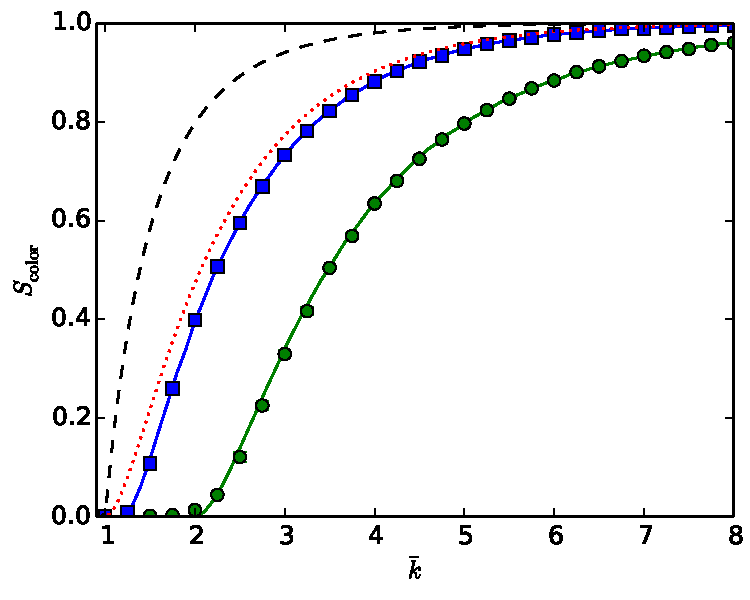
\includegraphics[width=1.0\columnwidth]{S_color_poisson.pdf}
    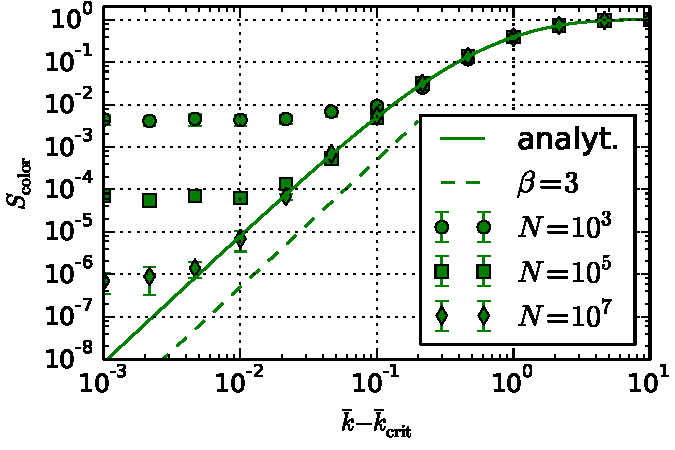
\includegraphics[width=1.0\columnwidth]{testtest.pdf}
    \caption{Top: Dependence of $S_{\rm color}$ on the average degree for Poisson graphs with different 
    numbers of colors. Symbols show numerical results for networks of size $N=1000$ 
    (blue squares for $C=10$ and green circles for $C=2$ colors), 
    the straight lines show the according analytical results. For comparison, 
    the giant component size $S$ is shown (black dashed). $S_{\rm color}$ is reduced due to two mechanisms: First, 
    every node has to be connected to the giant component via two links. The according fraction of 
    nodes $S_{{\rm color},\infty}$ is shown with a red dotted line. Second, increasing color frequencies 
    further decrease $S_{\rm color}$. Bottom: Finite size scaling for $C=3$ colors emphasizes the dependence 
    of the critical exponent $\beta$ on the color distribution, here $\beta=C=3$.}
    \label{fig:poisson}
\end{center}
\end{figure}
%%%
In figure~\ref{fig:poisson} on the top, the dependence of $S_{\rm color}$ on the average degree is shown for Poisson graphs 
with different numbers of colors $C$ (${\tilde r}_{c,k}=1/C$ is chosen homogeneous and independent of $k$). 
Comparing to the standard giant component size $S$ (dashed black line in the figure), 
the percolation sets in at increasing $\bar k$ with smaller numbers of colors, and the component size grows 
slower to the saturation value of one. The symbols show numerical results with $N=1000$ and 100 network realizations, 
the lines show results of equation~\ref{eq:s_color}, both correspond well. 

The suppression of the number of securely connected nodes can be understood as a combination of two effects. 
The first effect is purely topological and can be understood with $S_{{\rm color},\infty}$ of eq.~S\ref{eq:limit}
(shown with dotted red line). It means that only nodes can belong to $S_{\rm color}$, which are connected 
to the normal giant component over at least two links. We can confirm that 
$S_{\rm color}$ comes close to $S_{{\rm color},\infty}$ for high numbers of colors $C$ with the results for $C=10$.
$S_{{\rm color},\infty}$ is remarkably reduced compared to $S$ for small $k$, but has the same critical parameter. 
For the Poisson graph we show in the supplements that $S_{\rm color,\infty}\propto ({\bar k}-1)^2$ 
which grows slowly for small parameter ${\bar k}-1$. 

The second effect is connected to finite color frequencies ${\tilde r}_{c,k}$ which further reduces the percolating 
fraction of nodes. This also changes the critical value ${\bar k}_{\rm crit}$ and the critical exponent 
$\beta$. The critical behavior is discussed in detail in the supplements, for the general case of heterogeneous color 
distributions. Approximations in equation~\ref{eq:s_color} allow us to understand the critical behavior. 
Applied to the homogeneous color distributions discussed here, the results reduce to 
%%%
\begin{align}
S_{\rm color} &\propto ({\bar k}-{\bar k}_{\rm crit})^{\beta}\\
\beta&=C,\quad {\bar k}_{\rm crit} = C/(C-1).
\end{align}
%%%
This behavior can be confirmed with numerical results. On the bottom of the figure, a finite size 
scaling for $C=3$ colors establishes both the critical value of $3/2$ and the critical parameter.
For large numbers of colors, we observe the interesting phenomenon of high critical exponent 
$\beta$. With this, the system shows an effectively shifted transition between vanishing and finite $S_{\rm color}$, 
as the growth of the giant avoidable colors component 
$\frac{\rm d}{{\rm d} {\bar k}}S_{\rm color}\propto \beta ({\bar k}-{\bar k}_{\rm crit})^{\beta-1}$ 
is close to zero for small arguments. To our knowledge, this is a new kind of behavior, and a more 
detailed analysis of other quantities at the phase transition seems promising. 





\begin{figure}[htb]
\begin{center}
    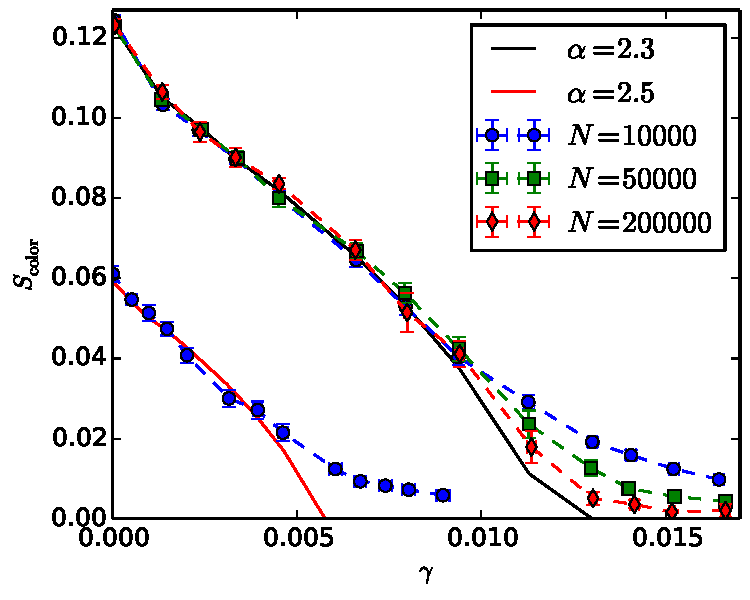
\includegraphics[width=1.0\columnwidth]{S_color_degree_dependent_broad.pdf}
    \caption{On graphs with broad degree distribution, $S_{\rm color}$ drops fast, 
    if a fraction $\gamma$ of nodes with the highest 
    degree is restricted to one color, while the nodes with smaller degree can have one of 
    two colors. This is shown for networks with $\alpha=2.3$ and $\alpha=2.5$ having $N=10000$ 
    with symbols. Analytical results need the modified version of equation~\ref{eq:s_color} 
    as described in section~\ref{subsec:degree}. Results are shown with straight lines. Without diversity 
    on the hubs, nodes cannot communicate in the desired way.}
    \label{fig:degree}
\end{center}
\end{figure}

Lets now discuss graphs with broad degree distributions with 
$p_k=n k^{-\alpha}$. $n$ is a normalization constant. 
For broad degree distributions, color distributions can show an additional type of 
heterogeneity, as a dependence of frequencies on the degree of a node can strongly 
influence the behavior. We used two colors, where the first color has a frequency 
of ${\tilde r}_{1,k}=1$ for all degrees $k\geq k_{\rm step}$ larger than a certain 
$k_{\rm step}$. These nodes have a probability of 
$\gamma=\sum_{k=k_{\rm step}}^{\infty} p_k$. Accordingly 
${\tilde r}_{2,k}=0$ for $k\geq k_{\rm step}$, and probabilities for smaller degrees are chosen as 
${\tilde r}_{c,k}=1/2$. Figure~\ref{fig:degree} shows results for an ensemble with 
$\alpha=2.3$ and $\alpha=2.5$. The analytical results for $\alpha=2.3$ show that already for a portion 
of $\gamma=1.4\%$ of the largest nodes occupied by the first color exclusively, $S_{\rm color}$ vanishes. 





\begin{figure}[htb]
\begin{center}
    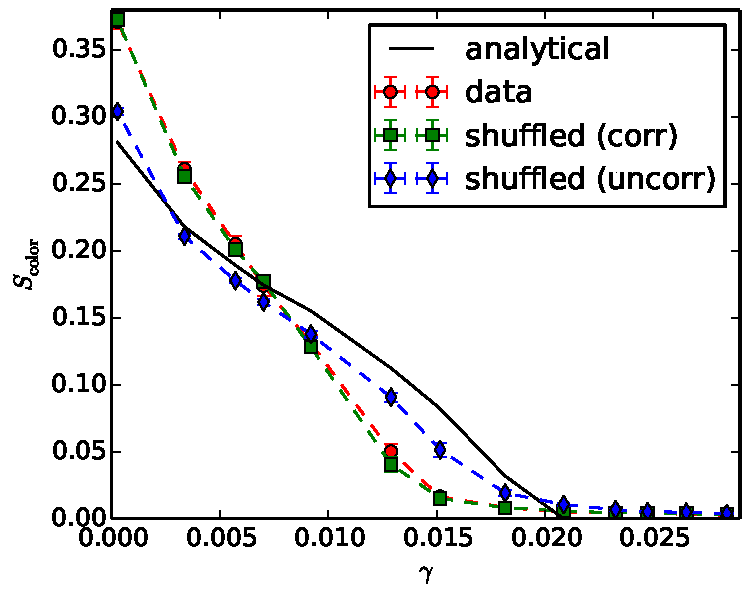
\includegraphics[width=1.0\columnwidth]{S_color_degree_dependent_data.pdf}
    \caption{Red circles show results for the network of autonomous systems, where colors are 
    distributed in the same way as in figure~\ref{fig:degree}. Averages were taken over 10 color 
    distributions. Analytical results are shown with the black line and reproduce the results qualitatively. 
    Deviations are due to degree-degree-correlations which are reserved in shuffled networks shown 
    with green squares, while results with ignoring correlations are shown with blue diamonds.}
    \label{fig:as}
\end{center}
\end{figure}

The red circles in figure~\ref{fig:as} show results for the autonomous systems network, where colors 
where distributed with degree-dependence over the nodes as described at the end of the last section. 
Averages where taken over 10 realizations of the color distributions. As expected from our results 
for scale free degree distributions, $S_{\rm color}$ drops to 0 even for small fraction $\gamma$ 
which is exclusively of one color. That means that if there is no heterogeneity in the highly 
connected servers, it is not possible to avoid e.g. software versions. This is also 
interesting in the following sense: It is known that secret services try to store all decrypted data 
running through servers to decrypt it later. As this is connected to technical afford, 
the services will more likely monitor the large servers. Therefore it would be beneficial, if once 
using encryption, to sent parts of the message using small servers. Unfortunately, this seems to 
be impossible, the services only have to monitor a low percentage of servers to hinder alternative 
paths. 

In order to assess the predictive power of our analytical method, we used a model ensemble with 
using the degree frequencies of the autonomous systems network as degree distribution $p_k$. 
Results for the according ensemble are shown with the black line. The qualitative 
behavior is represented well. To understand deviations, we compared to data from shuffled networks 
starting with the original data. Shuffling with ignoring degree-degree-correlations while only 
keeping the degree sequence gives results close to the analytical results (blue diamonds). 
Shuffling with also keeping degree-degree-correlations gives results close to the original network 
(green squares). 
Therefore, deviations between our theory and the data arise mainly due to degree-degree-correlations. 












\section{Summary and Outlook}








\bibliographystyle{apsrev4-1}
\bibliography{mp}

\end{document}
